\subsection{Актуальность работы}

\subsection{Организация и планирование работы}

Основные задачи организации и планирования работ:
\begin{itemize}
 \item определение объема предстоящих работ;
 \item определение основных этапов работ;
 \item установление сроков выполнения запланированных работ;
 \item определение необходимых денежных, материальных и трудовых ресурсов.
\end{itemize}


При выполнении дипломной работы были задействованы следующие лица:
\begin{itemize}
 \item руководитель (рук.);
 \item разработчик (разр.).
\end{itemize}

Месячный оклад студента, не являющегося дипломированным специалистом, составляет 2324,40 рублей.
С учетом 24 рабочих дней и 6-часового рабочего дня стоимость одного часа работ равна 16,14 рублей.
Месячный оклад руководителя с ученой степенью кандидата наук и должностью доцента составляет 14800 рублей.
Стоимость одного часа работ с учетом 24-ех 6-часовых рабочих дней равна 102,78 рублей.   

Руководитель работы оказывает помощь разработчику в планировании работ в период проектирования, рекомендует
необходимую литературу, проводит консультации разработчика, осуществляет контроль над выполнением всех 
намеченных этапов работы. Разработчик реализует объем работ, установленный в техническом задании.

График работ приведен в таблице~\ref{tab:job_is_done_1}.

\begin{table}[!ht]
\caption{График выполнения работ}
\centering
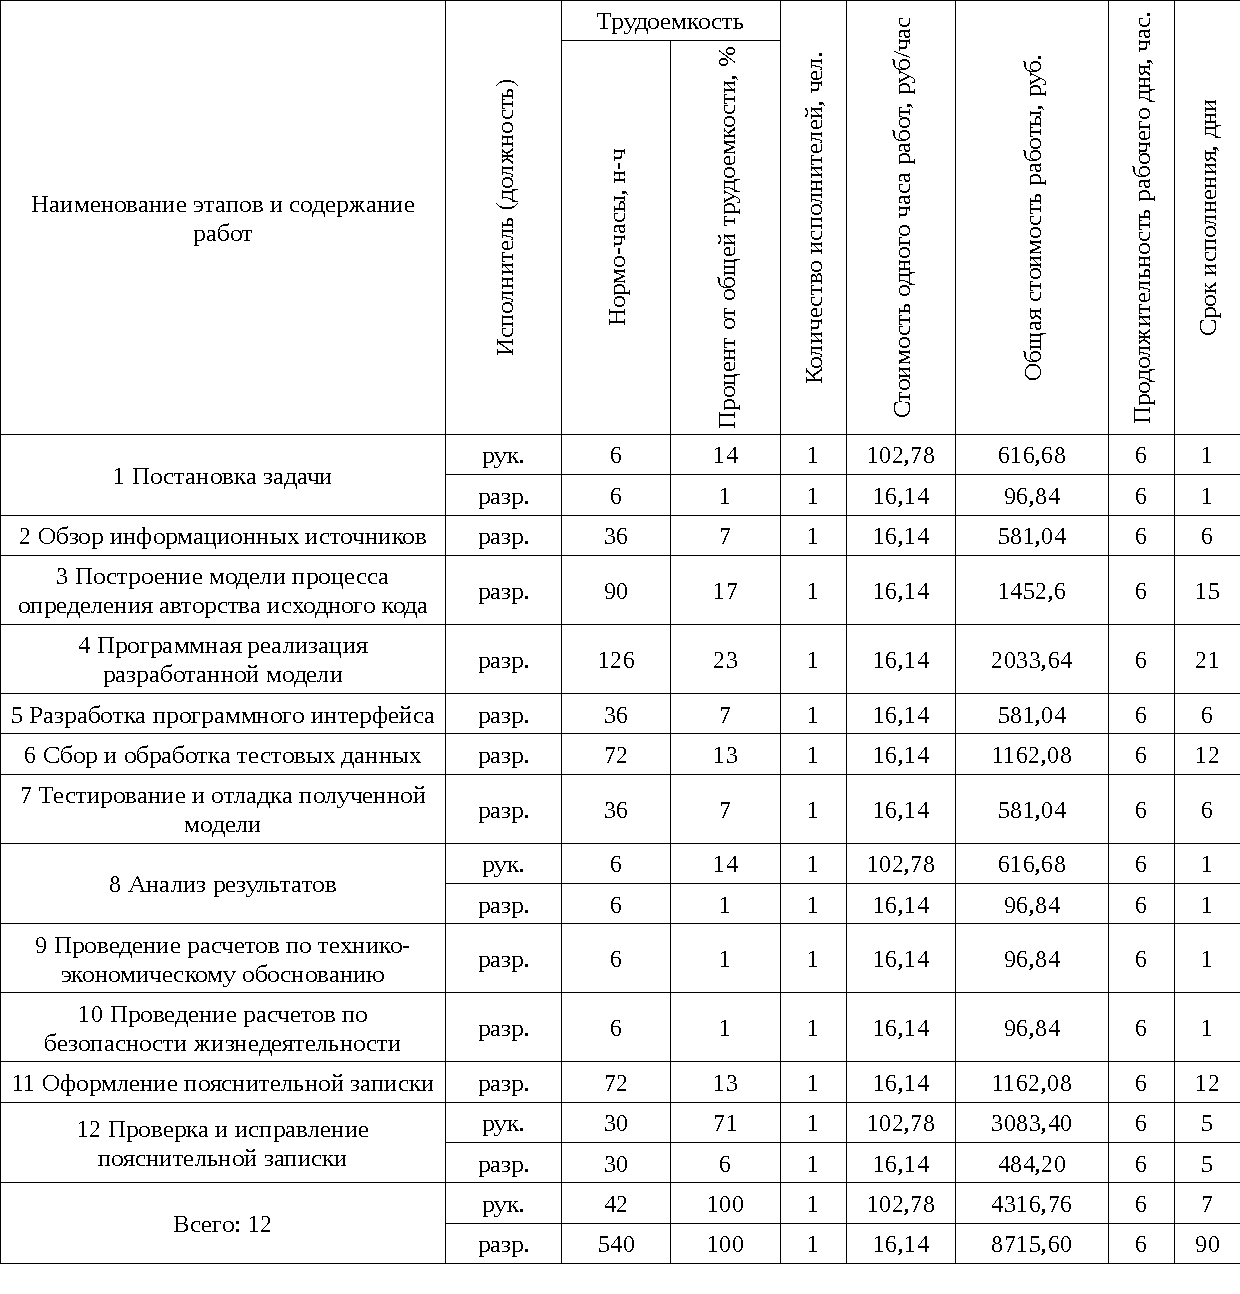
\includegraphics[page=1, width=1\linewidth]{economics_tables.pdf}
\label{tab:job_is_done_1}
\end{table}

\clearpage